% LaTeX source for textbook ``How to think like a computer scientist''
% Copyright (c)  2001  Allen B. Downey, Jeffrey Elkner, and Chris Meyers.

% Permission is granted to copy, distribute and/or modify this
% document under the terms of the GNU Free Documentation License,
% Version 1.1  or any later version published by the Free Software
% Foundation; with the Invariant Sections being ``Contributor List'',
% with no Front-Cover Texts, and with no Back-Cover Texts. A copy of
% the license is included in the section entitled ``GNU Free
% Documentation License''.

% This distribution includes a file named fdl.tex that contains the text
% of the GNU Free Documentation License.  If it is missing, you can obtain
% it from www.gnu.org or by writing to the Free Software Foundation,
% Inc., 59 Temple Place - Suite 330, Boston, MA 02111-1307, USA.
\chapter{Variables, expresiones y sentencias}

\section{Valores y tipos}
\index{valor}
\index{tipo}
\index{cadena}


Un {\bf valor} es una de las cosas fundamentales---como una letra o un 
número---que una progama manipula.  Los valores que hemos visto hasta ahorra
son \texttt{2} (el resultado cuando añadimos \texttt{1 + 1}, y
{\verb+"Hola todo el Mundo!"+}.

Los valores pertenecen a diferentes {\bf tipos}:
\texttt{2} es un entero, y {\verb+"Hola, Mundo!"+} es una {\bf cadena},
llamada así porque contiene una ``cadena'' de letras.
Usted (y el intérprete) pueden identificar cadenas porque  están
encerradas entre comillas.

La sentencia de impresión también trabaja con enteros.

\beforeverb
\begin{verbatim}
>>> print 4
4
\end{verbatim}
\afterverb
%
Si no está seguro del  tipo que un valor tiene,
el intérprete le puede decir.

\beforeverb
\begin{verbatim}
>>> type("Hola, Mundo!")
<type 'string'>
>>> type(17)
<type 'int'>
\end{verbatim}
\afterverb
%
Sin despertar ninguna sorpresa, las cadenas pertenecen al tipo \texttt{string (cadena)} y los enteros pertenecen al tipo \texttt{int}.  Menos obvio, los números con cifras decimales
pertenecen a un tipo llamado \texttt{float},
porque éstos se representan en un formato denominado
 {\bf punto flotante}.

\index{tipo}
\index{cadena}
\index{tipo!cadena}
\index{int}
\index{tipo!int}
\index{float}
\index{tipo!float}

\beforeverb
\begin{verbatim}
>>> type(3.2)
<type 'float'>
\end{verbatim}
\afterverb
%
¿Qué ocurre con valores como {\verb+"17"+} y {\verb+"3.2"+}?
Parecen números, pero están encerrados entre comillas como 
las cadenas.

\beforeverb
\begin{verbatim}
>>> type("17")
<type 'string'>
>>> type("3.2")
<type 'string'>
\end{verbatim}
\afterverb
%
Ellos son cadenas.

Cuando usted digita un número grande, podría estar tentado a usar
comas para separar grupos de tres dígitos, como en  \texttt{1,000,000}.  
Esto no es un número entero legal en Python, pero esto si es legal:

\beforeverb
\begin{verbatim}
>>> print 1,000,000
1 0 0
\end{verbatim}
\afterverb
%
¡Bueno, eso no es lo que esperábamos!.  Resulta que  {\tt
1,000,000} es una tupla, algo que encontraremos en el 
Capítulo \ref{tuplechap}.  De momento, recuerde no poner comas en sus 
números enteros.


\section{Variables}
\index{variable}
\index{asignación}
\index{sentencia!asignación}

Una de las características más poderosas en un lenguaje de programación
es la capacidad de manipular  {\bf variables}.  Una variable es un nombre
que se refiere a un valor.

La  {\bf sentencia de asignación} crea nuevas variables y les da valores:

\beforeverb
\begin{verbatim}
>>> mensaje = "¿Qué Onda?"
>>> n = 17
>>> pi = 3.14159
\end{verbatim}
\afterverb
%
Este ejemplo hace tres asignaciones: la primera asigna la cadena
{\verb+"¿Qué Onda?"+} a una nueva variable denominada \texttt{mensaje}, 
la segunda le asigna el entero \texttt{17} a \texttt{n} y la tercera le
asigna el número de punto flotante \texttt{3.14159} a \texttt{pi}.

\index{diagrama de estados}

Una manera común de representar variables en el papel es escribir el nombre
de la variable con una flecha apuntando a su valor. Esta clase de dibujo se
denomina  {\bf diagrama de estados} porque muestra el estado de cada una de 
las variables (piense en los valores como el estado mental de las variables).
Este diagrama muestra el resultado de las sentencias de asignación anteriores:

\beforefig
\centerline{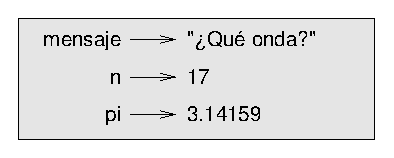
\includegraphics{illustrations/state2.eps}}
\afterfig

La sentencia \texttt{print} también funciona con variables.

\beforeverb
\begin{verbatim}
>>> print mensaje
Que Onda?
>>> print n
17
>>> print pi
3.14159
\end{verbatim}
\afterverb
%
En cada caso el resultado es el valor de la variable.
Las variables también tienen tipos; nuevamente, le podemos preguntar 
al intérprete cuales son.

\beforeverb
\begin{verbatim}
>>> type(mensaje)
<type 'string'>
>>> type(n)
<type 'int'>
>>> type(pi)
<type 'float'>
\end{verbatim}
\afterverb
%
El tipo de una variable es el mismo del valor al que se refiere.


\section{Nombres de variables y palabras reservadas}
\index{palabra reservada}
\index{palabra!reservada}

Los programadores, generalmente, escogen nombres significativos para
sus variables ---que especifiquen para qué se usa la variable.

Estos nombres pueden ser arbitrariamente largos. Pueden contener
letras y números, pero tienen que empezar con una letra. Aunque 
es legal usar letras mayúsculas, por convención no lo hacemos. Si
usted lo hace, recuerde que la capitalización importa, \texttt{Pedro}
y \texttt{pedro} son variables diferentes.

El carácter subrayado (\texttt{\_}) puede aparecer en un nombre. A menudo
se usa en nombres con múltiples palabras, tales como 
\texttt{mi\_nombre} ó \texttt{precio\_del\_café\_en\_china}.

\index{carácter subrayado}

Si usted le da un nombre ilegal a una variable obtendrá un error sintáctico:

\adjustpage{-2}
%\pagebreak
\beforeverb
\begin{verbatim}
>>> 76trombones = "gran desfile"
SyntaxError: invalid syntax
>>> mas$ = 1000000
SyntaxError: invalid syntax
>>> class = "introducción a la programación"
SyntaxError: invalid syntax
\end{verbatim}
\afterverb
%
\texttt{76trombones} es ilegal porque no empieza con una letra.

\texttt{mas\$} es ilegal porque contiene un  carácter ilegal, el símbolo \$. 

¿Qué sucede con \texttt{class}?

Resulta que \texttt{class} es una de las {\bf palabras reservadas (keywords)} de Python.
Las palabras reservadas definen las reglas del lenguaje y su estructura, y no 
pueden ser usadas como nombres de variables.

\index{palabra reservada}

Python tiene veintiocho palabras reservadas:

\beforeverb
\begin{verbatim}
and       continue  else      for       import    not       
assert    def       except    from      in        or        
break     del       exec      global    is        pass      
class     elif      finally   if        lambda    print     
raise     return    try       while
\end{verbatim}
\afterverb
%
Usted puede mantener esta lista a mano. Si el intérprete se queja 
por alguno de sus nombres de variables, y usted no sabe por qué,
búsquelo en esta lista.


\section{Sentencias}

Una sentencia es una instrucción que el intérprete de Python puede
ejecutar. Hemos visto dos clases de sentencias: la asignación y print.

Cuando usted digita una sentencia en la línea de comandos, Python la
ejecuta y despliega el resultado, si hay alguno. El resultado de un 
print es un valor. Las asignaciones no producen un resultado.

Un guión usualmente contiene una secuencia de sentencias. Si hay más 
de una, los resultados aparecen uno a uno a medida que las sentencias
se ejecutan.

Por ejemplo, el guión

\beforeverb
\begin{verbatim}
print 1
x = 2
print x
\end{verbatim}
\afterverb
%
produce la salida

\beforeverb
\begin{verbatim}
1
2
\end{verbatim}
\afterverb
%
Observe nuevamente que la sentencia de asignación no produce salida.



\section{Evaluando expresiones}

Una expresión es una combinación de valores, variables y operadores.
Si usted digita una expresión en la línea de comandos, el intérprete
la {\bf evalúa} y despliega su resultado:

\beforeverb
\begin{verbatim}
>>> 1 + 1
2
\end{verbatim}
\afterverb
%
Un valor, por si mismo, se considera como una expresión, lo mismo ocurre para las variables.

\beforeverb
\begin{verbatim}
>>> 17
17
>>> x
2
\end{verbatim}
\afterverb
%
Aunque es un poco confuso, evaluar una expresión no es lo mismo que imprimir o
desplegar un valor.

\beforeverb
\begin{verbatim}
>>> mensaje = "Como le va, Doc?"
>>> mensaje
"Como le va, Doc?"
>>> print mensaje
Como le va, Doc?
\end{verbatim}
\afterverb
%
Cuando  Python  muestra el valor de una expresión que
ha evaluado, utiliza el mismo formato que se usaría para entrar un valor. 
En el caso de las cadenas, esto implica que se incluyen las
comillas. Cuando se usa la sentencia print, el efecto es distinto 
como usted ya lo ha evidenciado.

En un guión, una expresión, por sí misma, es una sentencia legal, pero no 
realiza nada. El guión:

\beforeverb
\begin{verbatim}
17
3.2
"Hola, Mundo!"
1 + 1
\end{verbatim}
\afterverb
%
no produce ninguna salida. ¿Cómo cambiaría el guión 
de manera que despliegue los valores de las cuatro expresiones?


\section{Operadores y operandos}
\index{operador}
\index{operando}
\index{expresión}

Los {\bf operadores} son símbolos especiales que representan cómputos,
como la suma y la multiplicación. Los valores que el operador usa se denominan
{\bf operandos}.

Los siguientes son expresiones válidas en Python, cuyo significado es más o menos claro:
\adjustpage{2}
\beforeverb
\begin{verbatim}
20+32       hora-1   hora*60+minuto   
minuto/60   5**2     (5+9)*(15-7)
\end{verbatim}
\afterverb
%
Los  símbolos \texttt{+}, \texttt{-}, y \texttt{/}, y los paréntesis para
agrupar, significan en Python lo mismo que en la matemática.
El asterisco (\texttt{*}) es el símbolo para la multiplicación, y \texttt{**} es el  símbolo para la exponenciación.

Cuando el nombre de una variable aparece en lugar de un operando, se
reemplaza por su valor antes de calcular la operación

La suma, resta, multiplicación y exponenciación realizan lo que usted
esperaría, pero la división podría sorprenderlo.  La siguiente
operación tiene un resultado inesperado:

\beforeverb
\begin{verbatim}
>>> minuto = 59
>>> minuto/60
0
\end{verbatim}
\afterverb
%
El valor de \texttt{minuto} es 59, y 59 dividido por 60 es 0.98333,
no 0.  La razón para esta discrepancia radica en que Python está realizando
{\bf división entera}.

\index{división entera}

Cuando los dos operandos son enteros el resultado también debe ser un entero; y, por convención, la división entera siempre redondea {\em hacia abajo}, incluso en casos donde el siguiente entero está muy cerca.

Una solución posible a este problema consiste en calcular un porcentaje, en lugar de una fracción:

\beforeverb
\begin{verbatim}
>>> minuto*100/60
98
\end{verbatim}
\afterverb
%
De nuevo, el resultado se redondea; pero, al menos ahora, el resultado estará mas aproximado.  Otra alternativa es usar la división en punto
flotante, lo que haremos en el Capítulo \ref{floatchap}.


\section{Orden de las operaciones}
\index{orden de las operaciones}
\index{reglas de precedencia}

Cuando hay más de un operador en una expresión, el orden de
evaluación depende de las {\bf reglas de precedencia}.  Python sigue
las mismas reglas de precedencia a las que estamos acostumbrados para sus operadores matemáticos.
 El acrónimo {\bf PEMDAS} es útil para recordar el
orden de las operaciones:

\begin{itemize}

\item Los {\bf P}aréntesis tienen la precedencia más alta y pueden
usarse para forzar la evaluación de una expresión de la manera que usted
desee. Ya que las expresiones en paréntesis se evalúan primero, \texttt{2 * (3-1)} es 4, y \texttt{(1+1)**(5-2)} es 8. 
Usted también puede usar paréntesis para
que una expresión quede más legible, como en \texttt{(minuto * 100) / 60}, aunque 
esto no cambie el resultado.

\item La {\bf E}xponenciación tiene la siguiente precedencia más alta, así que
\texttt{2**1+1} es 3 y no 4, y \texttt{3*1**3} es 3 y no 27.

\item La {\bf M}ultiplicación y la {\bf D}ivisión tienen la misma precedencia,
aunque es más alta que la de la  {\bf A}dición y la  {\bf S}ubtracción, que también tienen la misma precedencia.  Así que  \texttt{2*3-1} da 5 en lugar de 4, y
\texttt{2/3-1} es \texttt{-1}, no \texttt{1} (recuerde que en división entera, \texttt{2/3=0}).

\item Los operadores con la misma precedencia se evalúan de izquierda
a derecha.  Recordando que \texttt{minuto=59},  en la expresión \texttt{minuto*100/60}; la multiplicación
se hace primero, resultando \texttt{5900/60}, lo que a su vez da \texttt{98}.
Si las operaciones se hubieran evaluado de derecha a izquierda, el resultado
sería \texttt{59/1}, que es \texttt{59}, y no es lo correcto.

\end{itemize}


\section{Operaciones sobre cadenas}
\index{operación sobre cadenas}

En general, usted no puede calcular operaciones matemáticas sobre cadenas,
incluso si las cadenas lucen como números. Las siguientes operaciones son 
ilegales (asumiendo que \texttt{mensaje} tiene el tipo \texttt{cadena}):

\beforeverb
\begin{verbatim}
 mensaje-1   "Hola"/123   mensaje*"Hola"   "15"+2
\end{verbatim}
\afterverb
%
Sin embargo, el operador \texttt{+} funciona con cadenas, aunque no calcula lo
que usted esperaría.  Para las cadenas, el operador \texttt{+}
representa la {\bf concatenación}, que significa unir los dos operandos 
enlazándolos en el orden en que aparecen. Por ejemplo:

\index{concatenación}

\beforeverb
\begin{verbatim}
fruta = "banano"
bienCocinada = " pan con nueces"
print fruta + bienCocinada
\end{verbatim}
\afterverb
%
La salida de este programa es  \texttt{banano pan con nueces}. El espacio
antes de la palabra \texttt{pan} es parte de la cadena y sirve para
producir el espacio entre las cadenas concatenadas.

El operador \texttt{*} también funciona con las cadenas; hace una repetición.
Por ejemplo, \texttt{'Fun'*3} es \texttt{'FunFunFun'}.  Uno de los operandos tiene que ser una cadena, el otro tiene que ser un entero.

Estas interpretaciones de \texttt{+} y \texttt{*} tienen sentido por la analogía
 con la suma y la  multiplicación.  Así como \texttt{4*3} es
equivalente a \texttt{4+4+4}, esperamos que \texttt{"Fun"*3} sea lo mismo que
{\verb/"Fun"+"Fun"+"Fun"/}, y lo és.  Sin embargo, las operaciones de concatenación y repetición 
sobre cadenas tienen una diferencia
significativa con las operaciones de suma y multiplicación.
¿Puede usted pensar en una propiedad que la suma y la multiplicación tengan
y que la concatenación y repetición no?



\section{Composición}
\index{composición}


Hasta aquí hemos considerado a los elementos de un programa---variables,
expresiones y sentencias---aisladamente, sin especificar cómo combinarlos.

Una de las características mas útiles de los lenguajes de programación es
su capacidad de tomar pequeños bloques para  {\bf componer} con ellos.  Por
ejemplo, ya que sabemos cómo sumar números y cómo imprimirlos; podemos hacer
las dos cosas al mismo tiempo:

\beforeverb
\begin{verbatim}
>>>  print 17 + 3
20
\end{verbatim}
\afterverb
%
De hecho, la suma tiene que calcularse antes que la impresión, así que las
acciones no están ocurriendo realmente al mismo tiempo. El punto es que  
cualquier expresión que tenga números, cadenas y variables puede ser usada
en una sentencia de impresión (\texttt{print}).  Usted ha visto un ejemplo 
de esto:

\beforeverb
\begin{verbatim}
print "Número de minutos desde media noche: ", 
      hora*60+minuto
\end{verbatim}
\afterverb
%
Usted también puede poner  expresiones arbitrarias en el lado derecho de
una sentencia de asignación:

\beforeverb
\begin{verbatim}
porcentaje = (minuto * 100) / 60
\end{verbatim}
\afterverb
%
Esto no parece nada impresionante ahora, pero vamos a ver otros ejemplos
en los que la composición hace posible expresar cálculos complejos organizada
y concisamente.

Advertencia: hay restricciones sobre los lugares en los que 
se pueden usar las expresiones. Por ejemplo, el lado izquierdo de una asignación tiene que ser
un nombre de {\em variable}, no una expresión.  Así que esto es ilegal:
\texttt{minuto+1 = hora}.


\section{Comentarios}
\index{comentario}


A medida que los programas se hacen más grandes y complejos, se vuelven más
difíciles de leer. Los lenguajes formales son densos; y, a menudo, es difícil
mirar una sección de código y saber qué hace, o por qué lo hace.

Por esta razón, es una muy buena idea añadir notas a sus programas para
explicar, en lenguaje natural, lo que hacen. Estas notas se denominan
{\bf comentarios }y se marcan con el símbolo \texttt{\#}:

\beforeverb
\begin{verbatim}
# calcula el porcentaje de la hora que ha pasado
porcentaje = (minuto * 100) / 60
\end{verbatim}
\afterverb
%
En este caso, el comentario aparece en una línea completa. También pueden ir comentarios al final de una línea:

\beforeverb
\begin{verbatim}
# precaucion: division entera
porcentaje = (minute * 100) / 60   
\end{verbatim}
\afterverb
%
Todo lo que sigue desde el \texttt{\#} hasta el fin de la línea se ignora---no 
tiene efecto en el programa. El mensaje es para el programador que escribe
el programa o para algún programador que podría usar este código en el futuro.
En este caso, le recuerda al lector el sorprendente comportamiento de la 
división entera en Python.


\section{Glosario}

\begin{description}

\item[Valor:]  un número o una cadena (u otra cosa que se introduzca más adelante) que puede ser almacenado en una variable o calculado en una expresión.

\item[Tipo:]  conjunto de valores.  El tipo del valor determina cómo se puede usar en expresiones.  Hasta aquí, los tipos que usted ha visto son enteros (tipo \texttt{int}), números de punto flotante (tipo \texttt{float})
y cadenas (tipo \texttt{string}).

\item[Punto flotante:] formato para representar números con parte decimal.

\item[Variable:]  nombre que se refiere a un valor.

\item[Sentencia:]  sección de código que representa un comando o acción. 
Hasta aquí las sentencias que usted ha visto son la de asignación y 
la de impresión.

\item[Asignación:]  corresponde a la sentencia que pone un valor en una variable.

\item[Diagrama de estados:]  es la representación gráfica de un conjunto de
variables y los valores a los que se refieren.

\item[Palabra reservada:]  es una palabra usada por el compilador
para analizar sintácticamente un programa; usted no puede usar palabras reservadas 
como \texttt{if}, \texttt{def}, y \texttt{while} como nombres de variables.

\item[Operador:]  símbolo especial que representa un simple cálculo como
una suma, multiplicación o concatenación de cadenas.

\item[Operando:]  uno de los valores sobre el cual actúa un operador.

\item[Expresión:]  combinación de variables, operadores y valores que 
representa un único valor de resultado.

\item[Evaluar:]  simplificar una expresión ejecutando varias operaciones a fin
de retornar un valor único.

\item[División entera:]  operación que divide un entero por otro
y retorna un entero. La división entera retorna el número de veces que 
el denominador cabe en el numerador y descarta el residuo.

\item[Reglas de precedencia:] reglas que gobiernan el orden en que
las expresiones que tienen múltiples operadores y operandos se evalúan.

\item[Concatenar:]  unir dos operandos en el orden en que aparecen.

\item[Composición:]  es la capacidad de combinar simples expresiones y sentencias
dentro de sentencias y expresiones compuestas para representar cálculos complejos
concisamente.

\item[Comentario:]  información que se incluye en un programa para 
otro programador (o lector del código fuente) que no tiene efecto en la ejecución.


\index{valor}
\index{punto flotante}
\index{variable}
\index{tipo}
\index{palabra reservada}
\index{sentencia}
\index{asignación}
\index{comentario}
\index{diagrama de estados}
\index{expresión}
\index{operador}
\index{operando}
\index{división entera}
\index{reglas de precedencia}
\index{precedencia}
\index{concatenación}
\index{composición}

\end{description}

\section{Ejercicios}


\begin{enumerate}

\item Registre qué sucede cuando usa la sentencia print en combinación con una 
sentencia de asignación, por ejemplo \verb+print n = 7+.

\item ¿Que sucede cuando se usa la sentencia print con una expresión,  por ejemplo
\verb# print 8+5 #  ?

\item ¿Que sucede cuando se ejecuta esto? 

\verb+ print 5.2, "esto", 4 - 2, "aquello", 5/2.0 +

\item Tome la siguiente oración: Sólo trabajo y nada de juegos hacen de Juan un 
niño aburrido. Almacene cada palabra en variables separadas, después muestre la oración 
en una sola línea usando la sentencia print.

\item Incluya paréntesis a la expresión 6 * 1 - 2 para cambiar su resultado de 4 a -6.

\item Inserte una línea de comentario en un línea previa a una de código funcional, y 
registre qué es lo que sucede cuando corre de nuevo el programa.

\item La diferencia entre la función input y la función raw\_input es que la función 
input evalúa la cadena introducida y la función raw\_input no lo hace. Escriba lo siguiente 
en el intérprete de Python, registre qué sucede y expliquelo:

\begin{verbatim}
>>> x = input()
3.14
>>> type(x)
\end{verbatim}

\begin{verbatim}
>>> x = raw_input()
3.14
>>> type(x)
\end{verbatim}

\item Escriba una expresión que calcule la nota definitiva de su curso de programación.

\end{enumerate}
